\documentclass[12pt]{article}

\usepackage{sbc-template}

\usepackage{graphicx,url}

\usepackage[brazil]{babel} 
  
\usepackage[utf8]{inputenc}       

\usepackage{lipsum}

\sloppy

\title{Evoluç\~{a}o do Hardware dos consoles e seus periféricos}

\author{Henrique Shodi Maeta e Luiz Frederico}


\address{{Centro Universit\'{a}rio Senac, Santo Amaro}
\email{japa1996@hotmail.com}}

\begin{document} 

\maketitle

\begin{abstract}

  
\end{abstract}
     
\begin{resumo} 
\end{resumo}


\section{Introdu\c c\~{a}o}

\ \ A história dos consoles começam quando os cientistas da computaç\~{a}o iniciam suas pesquisas nas áreas de Inteligencia artificial, simuladores, computaç\~{a}o grafica entre outros.
 
 O primeiro video game, segundo o artigo "From Pong to Playstation 3" \cite{pong-play} foi projetado em 1948 quando Thomas T. Goldsmith Jr. (americano pioneiro no ramo da televis\~{a}o e professor de física na Furman University) e Estle Ray Mann emitiram uma patente americana para um "Despositivo para divers\~{a}o de tubo de raios catódicos", que era uma maquina com uma maçaneta para mirar e um bot\~{a}o para atirar em alvos de avi\~{o}es inspirada no radar, um dispositivo usado na Segunda Guerra Mundial. Mas por conta do custo do equipamento este projeto nunca foi fabricado, apenas surgiram poucos protótipos de fabricaç\~{a}o caseira inspirados neste projeto.
 Dez anos após o primeiro projeto o físico americano William A. Higinbotham, que participou da equipe que desenvolveu a primeira bomba nuclear, criou o Tennis for Two (Tênis para dois), que era um jogo onde um computador analógico era adicionado a um ociloscopio:
\linebreak
\begin{figure}[!htb]
    \centering
    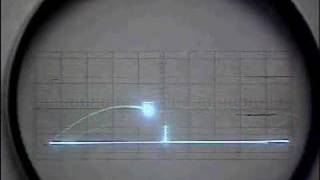
\includegraphics[width=0.8\textwidth]{osciloscopio.jpg}
    \caption{Imagem do jogo Tennis for Two no osciloscópio.}
    \label{fig:osciloscopio}
\end{figure}
\linebreak
 Os jogadores possuiam um bot\~{a}o para regular o ângulo que a bola iria seguir, e um bot\~{a}o para acertar a bola.
 
 Em 1961 um grupo de estudantes do MIT (Massachusetts Institute of Technology) escreveram o código de um jogo para o computador que eles possuiam DEC PDP-1, tal jogo foi nomeado Spacewar!. O jogo se baseava em duas naves espaciais (jogadores) que atiravam, e, o objetivo era derrotar a nave do outro jogador. 
\linebreak
\begin{figure}[!htb]
    \centering
    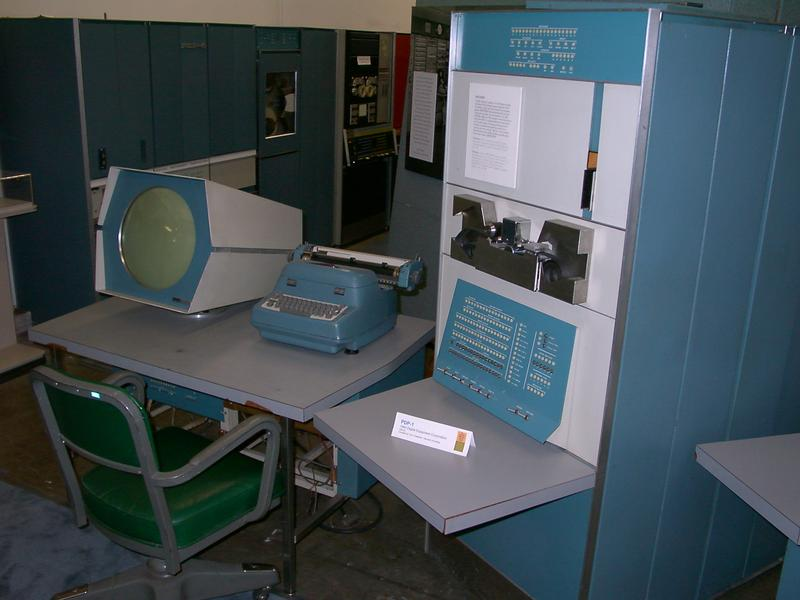
\includegraphics[width=0.8\textwidth]{pc-velho.jpg}
    \caption{Computador DEC PDP-1 mesmo modelo que os alunos utilizaram para programar Spacewar!}
    \label{fig:pc-velho}
\end{figure}
\linebreak
\begin{figure}[!htb]
    \centering
    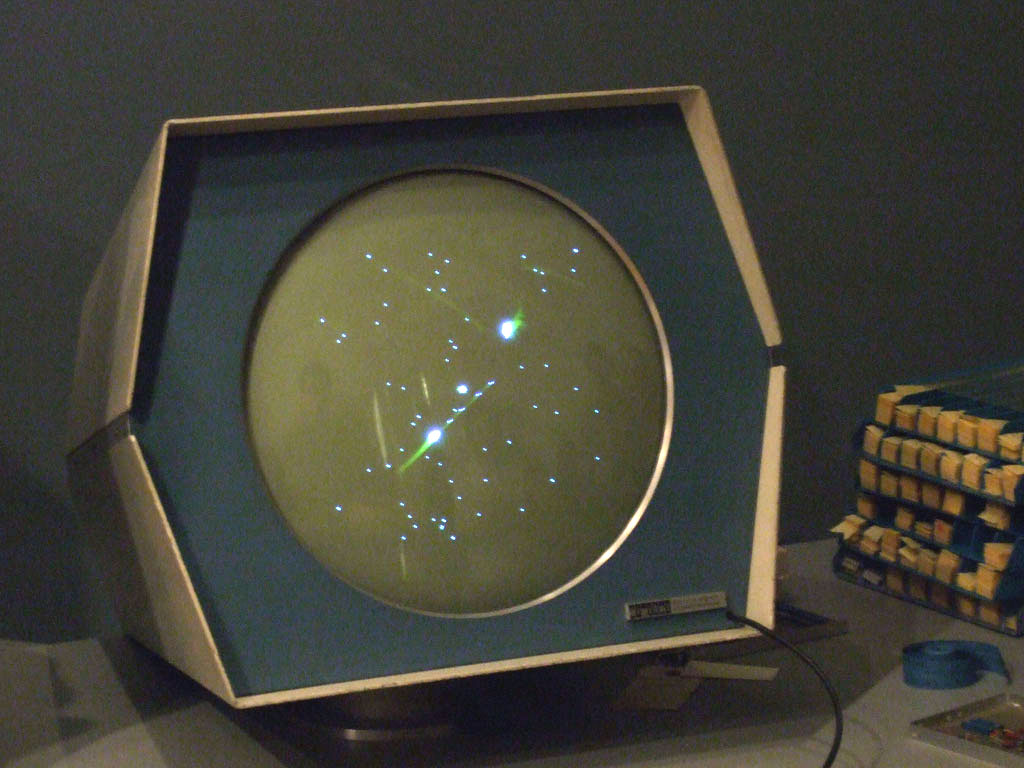
\includegraphics[width=0.6\textwidth]{spacewar.jpg}
    \caption{Imagem do jogo Spacewar!, onde os pontos verdes representam os jogadores.}
    \label{fig:spacewar}
\end{figure}
\linebreak
\pagebreak





 
\section{Algoritmo RSA}

\lipsum{2}

\section{Conclus\~{a}o}



\bibliographystyle{sbc}
\bibliography{sbc-template}
\nocite{pc-velho}
\end{document}
